\chapter{Exploration of energy efficient memory organisations for dynamic multimedia applications using system scenarios}

\begin{center}
Iason Filippopoulos, Francky Catthoor and Per Gunnar Kjeldsberg
\\
Memory Architecture and Organization Workshop
\\
Embedded Systems Week
\\
2013
\end{center}
\afterpage{\null\newpage}
\newpage

\vspace*{\fill}
%\addcontentsline{toc}{section}{Abstract}
\section*{\hspace*{\fill} Abstract \hspace*{\fill}}
We propose a memory-aware system scenario approach that exploits variations in memory needs during the lifetime of an application in order to optimize energy usage. Different system scenarios capture the application's different resource requirements which change dynamically at run-time. In addition to computational resources, the many possible memory platform configurations and data-to-memory assignments are important system scenario parameters. Here we present an extended memory model that includes existing state-of-the-art memories, available in the industry and academia, and show how it is employed during the system design exploration phase. Both commercial SRAM and standard cell based memory models are explored in this study. The effectiveness of the proposed methodology is demonstrated and tested using a large set of multimedia benchmarks published in the Polybench, Mibench and Mediabench suites. Reduction in energy consumption in the memory subsystem ranges from 35\% to 55 \% for the chosen set of benchmarks.
\vspace*{\fill}
\afterpage{\null\newpage}
\newpage

\section{Introduction}
%\label{sec:introduction}

Modern embedded systems are becoming more and more powerful as the semiconductor processing techniques keep increasing the number of transistors on a single chip. Consequentially, demanding applications, e.g., in the signal processing and multimedia domains, can be executed on these devices \cite{narasinga}. On the other hand, the desired performance has to be delivered with minimum power consumption due to the limited energy available in mobile devices \cite{tcm}. System scenario methodologies propose the use of different platform configurations in order to exploit run-time variations in computational and memory needs often seen in such applications \cite{tcm}.

%Francky: explain about the knobs
Platform reconfiguration is performed through tuning of different system parameters, also called system knobs. For the memory-aware system scenario methodology, a platform can be reconfigured through a number of potential knobs, each resulting in different performance and power consumption in the memory subsystem. Foremost, modern memories support different energy states, e.g., through power gating techniques and by switching to lower power modes when not accessed. %removed for blind \cite{Fil12}
The second platform knob is the assignment of data to the available memory banks. The data assignment decisions affect both the energy per access for the mapped data, the data conflicts as a result of suboptimal assignment, and the number of active banks. In this work a reconfigurable memory platform is constructed using detailed memory models. This is followed by experiments with dynamic multimedia applications in order to study the effectiveness of the methodology.

%Domain specific for ESTIMedia + comparison with use case
%in comparison with \cite{Fil12} 
%, which is potentially applicable to every multimedia application with dynamic memory usage. 
The main contribution of the current work is the development of data variable based system scenarios. Previous control variable based system scenarios are unable to handle the fine-grain behaviour of the studied multimedia applications due to their significant variation under different execution situations. Furthermore, compared with use case scenario approaches in which scenarios are generated based on a user's behaviour, the system scenario methodology focuses on the behaviour of the system to generate scenarios and can, therefore, fully exploit the detailed platform mapping information. Rather than focusing on the processing cores, this work analyses the application of system scenarios on the memory organisation. Other contributions are for the purpose sufficiently detailed and accurate memory models used for the system design exploration, an extensive number of benchmark applications on which the methodology is applied, and a categorisation of applications based on their dynamic characteristics. For the multimedia domain, the current work presents a comprehensive methodology for optimising energy consumption in the memory subsystem.

%It still means we can have measurable differences,
%in particular that we are exploiting data variable system scenarios (that - the data variables
%exploit detailed platform mapping information) instead
%of control variable sys-scen (which cannot handle our applications due
%to too fine grain scenario behaviour in the data variables) or use case scen
%(which do not exploit any detailed platform mapping info).
%And compared to the limited work that targets data variable sys-scen, we
%now focus on memory organ instead of the processor cores.
%I assume you can formulate a few sentences around the above?
%Most of the dynamic variables in the current work can be classified as data variables due to their significant variation under different execution situations. 

%This paper is organized as follows. Section~\ref{sec:motivation} motivates the study of optimization of the memory organisation and surveys related work on system level memory exploration. Section~\ref{sec:methodology} presents the chosen methodology with main focus on the memory organisation study. In Section~\ref{sec:platform} the target platform is described accompanied by a detailed description of the employed memory models, while the multimedia benchmarks and their characteristics are analysed in Section~\ref{sec:applications}. Results of applying the described methodology to the targeted applications are shown in Section~\ref{sec:results}, while conclusions are drawn in Section~\ref{sec:conclusion}. 

\section{Motivation and Related Work}
%\label{sec:motivation}

A large number of papers have demonstrated the importance of the memory organization to the overall system energy consumption. Especially for embedded systems, the memory subsystem accounts for up to 50\% of the overall energy consumption \cite{Che09} and the cycle-accurate simulator presented in \cite{Ben99} estimates that the energy expenditures in the memory subsystem range from 35\% up to 65\% for different architectures. According to \cite{tcm}, conventional allocation and assignment of data done by regular compilers is suboptimal. Performance loss is caused by stalls for fetching data and data conflicts for different tasks, due to the limited size of memory and the competition between tasks.The significant contribution that the memory subsystem has to the overall energy consumption of a system and the dynamic nature of many applications offer a strong motivation for the study and optimization of the memory organisation in modern embedded devices.

Many papers have focused on memory related optimisations, also in the presence of a partitioned and distributed memory organisation with memory blocks of different sizes. In \cite{Ben00b} authors present a methodology for automatic memory hierarchy generation that exploits memory access locality, while in \cite{Ben00c} they propose an algorithm for the automatic partitioning of on-chip SRAM in multiple banks. Several design techniques for designing energy efficient memory architectures for embedded systems are presented in \cite{Mac02}. The current work differentiates by employing a platform that is reconfigurable during run-time. In \cite{Pgk01} a large number of data and memory optimisation techniques, that could be dependent or independent of a target platform, are discussed. Again, reconfigurable platforms are not considered.

Energy-aware assignment of data to memory banks for several task-sets based on the MediaBench suit of benchmarks is presented in \cite{Mar03}. Low energy multimedia applications are discussed also in \cite{Chu02} with focus on processing rather than the memory platform. Furthermore, both \cite{Mar03} and \cite{Chu02} base their analysis on use case situations and do not incorporate sufficient support for very dynamically behaving application codes. System scenarios alleviate this bottleneck and enable handling of such dynamic behaviour. In addition, the current work explores the assignment of data to the memory and the effect of different assignment decisions on the overall energy consumption.

%An overview of work on system scenario methodologies and their application are presented in \cite{Gheorghita2007}. In \cite{Fil12} extensions towards a memory-aware system scenario methodology are presented and demonstrated using theoretical memory models and two target applications. This work is an extension both in complexity and accuracy of the considered memory library and on the number of target applications. 

\section{Data Variable Based Memory-Aware System Scenario Methodology}
%\label{sec:methodology}
%PKG: Remove most of the citations to Norchip

%The memory-aware system scenario methodology is based on the observation that the memory subsystem requirements at run-time vary significantly due to dynamic variations of memory needs in the application code. Most existing design methodologies define the memory requirements as that of the most demanding task and tune the system in order to meet its needs \cite{tcm}. Obviously, this approach leads to unused memory area for tasks with lower memory requirements, since those tasks could meet their needs using fewer resources and consequentially consuming less energy. Another source of unnecessary waste of energy in the memory is caused by data conflicts due to misplaced data. Replacement of old data and fetching of new data is both time and energy consuming and should therefore be avoided. Handling of data conflicts is also part of a memory-aware system scenario methodology.

Designing with system scenarios is workload adaptive and offers different configurations of the platform and the freedom of switching to the most efficient scenario at run-time. A system scenario is a configuration of the system that combines similar run-time situations (RTSs). An RTS consists of a running instance of a task and its corresponding cost (e.g., energy consumption) and one complete run of the application on the target platform represents a sequence of RTSs \cite{Elena2010}. The system is configured to meet the cost requirements of an RTS by choosing the appropriate system scenario, which is the one that satisfies the requirements using minimal power. In the following subsections, the different steps of the memory-aware system scenario methodology are outlined. 

The general system scenario methodology follows a two stage exploration, namely design-time and run-time stages, as described in \cite{Gheorghita2007}. This splitting is also employed in the memory-aware extension of the methodology. The two stage exploration is chosen because it reduces run-time overhead while preserving an important degree of freedom for run-time configuration \cite{tcm}. The application is analysed at design-time and different execution paths causing variations in memory demands are identified. This procedure, which is time consuming and as a result can be performed only during the design phase, will result in a grey-box model representation of the application. The grey-box model hides all static and deterministic parts of the application, by providing only related memory costs for those, and keeps parts of the application code that are non-deterministic in terms of memory usage available to the system designer \cite{graybox}. 


\subsection{Design-time Profiling Based on Data Variables}

\begin{figure}[!t]
\centering
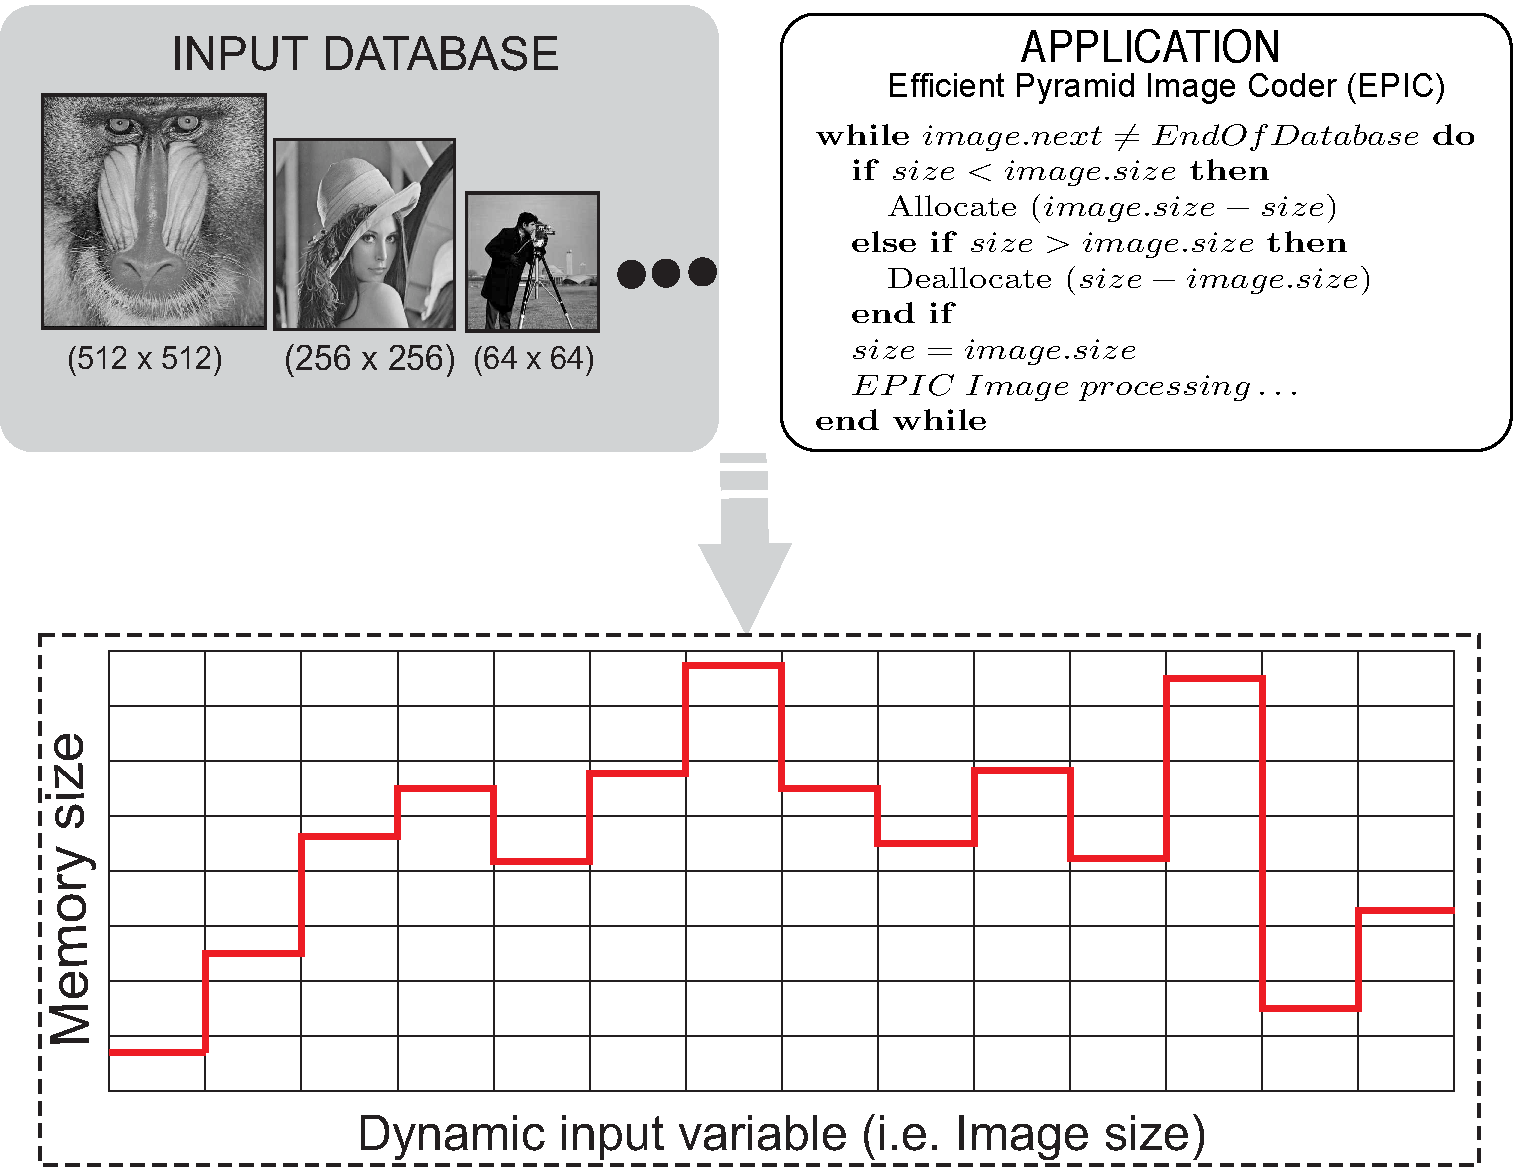
\includegraphics[width=\textwidth]{B/Images/profiling2.pdf}
\caption{Profiling results based on application code and input data}
\label{fig:profiling}
\end{figure}

Application profiling is performed at design-time for a wide range of inputs. The analysis focuses on the allocated memory size during execution and on access pattern variations. Techniques described in \cite{Ang13b} are, e.g., used in order to extract the access scheme through analysis of array iteration spaces.  

The profiling stage is depicted in Fig.~\ref{fig:profiling} and consists of running the application code with suitable input data often found in a database, in order to produce profiling results. The results shown here are limited for demonstrational purposes. A real application would have thousands or millions of profiling samples. The profiling reveals parts of the application code with high memory activity and with varying memory access intensity, which possibly depends on input data variables. Because of this behaviour, a static study of the application code alone is insufficient since the target applications for this methodology have non-deterministic behaviour that is driven by input.

%Given code and database with data inputs, profiling will show memory usage during run-time.
%% PGK suggests deleting: by running the application using the whole database as an input. 
%Results provided to the designer include complete information about allocated memory size values together with the number of occurrences and duration for each of these memory size values. Moreover, correlation between input data variable values and the resulting memory behaviour can possibly be observed. This information is useful for the clustering step that follows. 

In Fig.~\ref{fig:profiling} the profiled applications are two image related multimedia benchmarks and the input database should consist of a variety of images. The memory requirements in each case are driven by the current input image size, which is classified as a data variable due to the wide range of its possible values. Depending on the application the whole image or a region of interest is processed. 
Other applications have other input variables deciding the memory requirement dynamism, e.g., the SNR level on the channel in the case of an encoding/decoding application.

\subsection{Design-time System Scenario Identification and Prediction Based on Data Variables}

\begin{figure}[!t]
\centering
\includegraphics[width=\textwidth]{B/Images/1DclusteringShort.pdf}
%\includegraphics[angle=270, width=0.47\textwidth]{Images/1Dclustering.ps}
\caption{Clustering of profiling results into three (a) or five (b) system scenarios}
\label{fig:clustering}
\end{figure}

The next step is the clustering of the profiled memory sizes into groups with similar characteristics. This is referred to as system scenario identification. Clustering is necessary, because it will be extremely costly to have a different scenario for every possible size, due to the number of memories needed. Clustering neighbouring RTSs is a rational choice, because two instances with similar memory needs have similar energy consumption. In Fig.~\ref{fig:clustering} the clustering of the previously profiled information is presented. The clustering of RTSs is based both on their distance on the memory size axis and the frequency of their occurrence. Consequently, the memory size is split unevenly with more frequent RTSs having a shorter memory size range. This is better than even splitting because the energy cost of each system scenario is defined by the upper size limit, as each scenario should support all RTSs within its range. With more scenarios, e.g., five instead of 3, the aggregated RTS running overhead is reduced. Still the number of scenarios should be limited due to overhead of a complex memory platform and of frequent switching between scenarios.

The design-time system scenario prediction phase consists of determination of the data variables that define the active system scenario. This can be achieved by careful study of the application code, combined with the application's data input. In our case the grey-box model reveals only the code parts that will influence memory usage, so that data variables deciding memory space changes can be identified. An example of this is a non static variable that influences the number of iterations for a loop that performs one memory allocation at each iteration. In the depicted example the system scenario prediction data variable is the input image height and width values. Moreover, the designer should look for a correlation between input values and the corresponding cost. This information will be useful in the following steps of the methodology \cite{tcm}.


\subsection{Run-time System Scenario Detection and Switching Based on Data Variables}

Switching decisions are taken at run-time by the run-time manager. The switching phase consists of all platform configuration decisions that can be made at run-time, e.g., frequency/voltage scaling, changing the power mode of memory units, including turning them off, and reassignment of data on memory units. Switching takes place when the switching cost is lower than the energy gains achieved by switching. In more detail, the run-time manager compares the memory energy consumption of executing the next task in the current active system scenario with the energy consumption of execution with the optimal system scenario. If the difference is greater than the switching cost, then scenario switching is performed \cite{tcm}. Switching costs are defined by the platform and include all memory energy penalties for run-time reconfigurations of the platform, e.g., extra energy needed to change state of a memory unit.

\begin{figure}[!t]
\centering
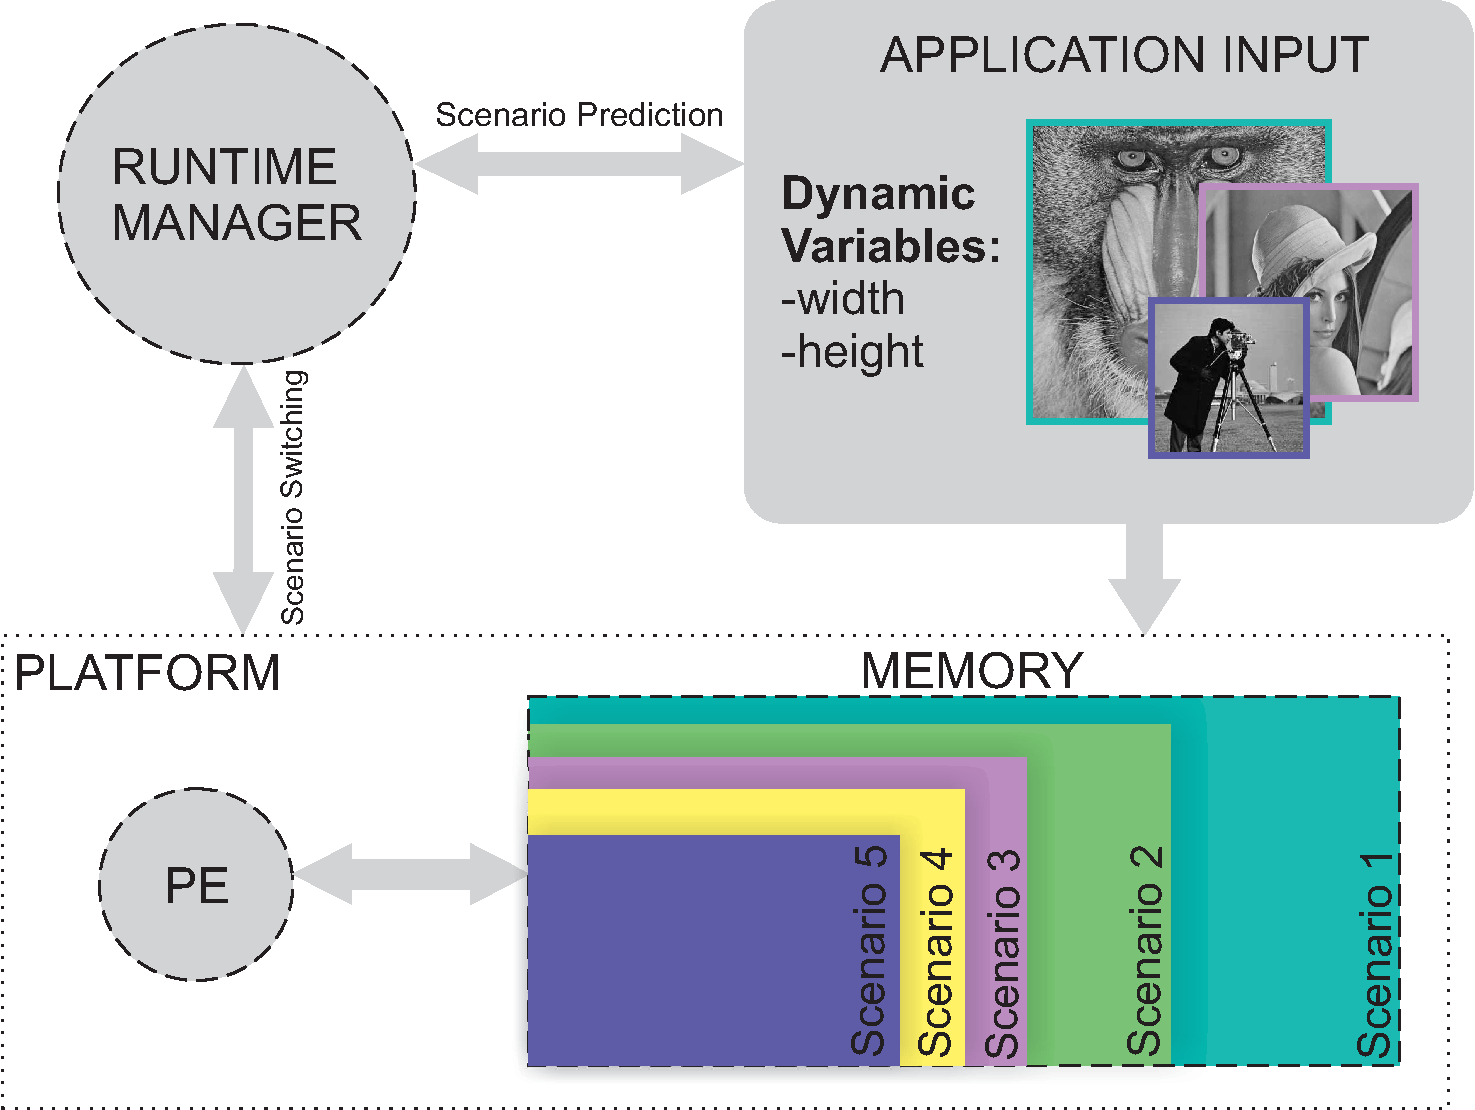
\includegraphics[width=\textwidth]{B/Images/switching.pdf}
\caption{Run-time system scenario prediction and switching based on the current input}
\label{fig:runtime}
\end{figure}

In Fig.~\ref{fig:runtime} an example of the run-time phase of the methodology is depicted. The run-time manager identifies the size of the image that will be processed and reconfigures the memory subsystem on the platform, if needed, by increasing or decreasing the available memory size. The reconfiguration options are effected by platform hardware limitations. The image size is the data variable monitored in order to detect the system scenario and the need for switching.

\section{Target Platform and energy models}
%\label{sec:platform}

Selection of target platform is an important aspect of the memory-aware system scenario methodology. The key feature needed in the platform architecture is the ability to efficiently support different memory sizes that correspond to the system scenarios generated by the methodology. The dynamic memory platform is achieved by organising the memory area in a varying number of banks that can be switched between different energy states. In this work, a clustered memory organisation with up to five memory banks of varying sizes is explored. Some examples of alternative memory platforms that can be used for exploration is shown in Fig.~\ref{fig:platform}.

\begin{figure}[!t]
\centering
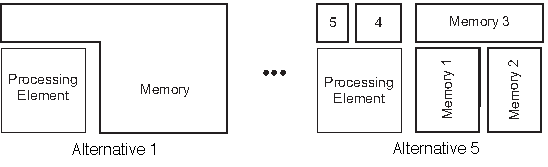
\includegraphics[width=\textwidth]{B/Images/platform.pdf}
\caption{Alternative memory platforms with varying number of banks}
\label{fig:platform}
\end{figure}

%For more complex architectures the interconnection cost should be considered and analysed separately for accurate results. Although power gating can be applied to the bus when only a part of a longer bus is needed, an accurate model of the memory wrapper and interconnection must developed, which is beyond the scope of the current work.  Point-to-point connections with negligible interconnect costs between elements are assumed for up to five memory banks.

\subsection{Models of Different Memory Types}

The dynamic memory organisation is constructed using commercially available SRAM memory models (MM). In addition, experimental standard cell-based memories (SCMEM) \cite{Mei11}  are  considered for smaller memories due to their energy and area efficiency for reasonably small storage capacities, as argued in \cite{Mei10}. Both MMs and SCMEMs can operate under a wide range of supply voltages, thus support different operating modes that provide an important exploration space. In the active mode the memory can be accessed at the maximum supported speed and the supply voltage is set at 1.1V. While data are not accessed for a period of time the light/deep sleep or shut down mode should be considered. In light sleep mode the supply voltage is lowered with values around 0.7V, while on deep sleep mode the supply voltage is set to the lowest possible value that can be used without loss of data. This voltage threshold is expected to be lower for SCMEMs than MM models and can be as low as 0.3V. The shut down mode uses power-gating techniques to achieve near zero leakage power, but stored data is lost. The time and the energy required for switching from these low leakage modes to the active state differs and all the necessary energy/power information is available to the system designer.

\subsection{Energy consumption calculation}
The overall energy consumption for each configuration is calculated using a detailed formula, as can be seen in (\ref{eq:energy}). 
%\setlength{\arraycolsep}{0.0em}
%\begin{eqnarray}
%\label{eq:energy}
% E &{}= {}&\sum\limits_{memories}^{all}  ( N_{rd} \times E_{Read} \nonumber\\
%		&&+ N_{wr} \times E_{Write} \nonumber\\
%		&&+ (T-T_{LSleep}-T_{DSleep}-T_{ShutDown})\times P_{leak_{Active}} \nonumber\\
%		&&+ T_{LSleep} \times P_{leak_{LSleep}} \nonumber\\
%		&&+ T_{DSleep} \times P_{leak_{DSleep}} \nonumber\\
%		&&+ T_{ShutDown} \times P_{leak_{ShutDown}} \nonumber\\ 
%		&& + N_{SWLight} \times E_{LSleep \: to \: Active} \nonumber\\
%		&& + N_{SWDeep} \times E_{DSleep \: to \: Active} \nonumber\\
%		&& + N_{SWShutDown} \times E_{ShutDown \: to \: Active} ) \nonumber\\
%\end{eqnarray}
%\setlength{\arraycolsep}{5pt}
\begin{equation}
\label{eq:energy}
\begin{array}{lcl}
E&=&\sum\limits_{memories}^{all}  ( N_{rd} \times E_{Read}+ N_{wr} \times E_{Write}\\
&+&(T-T_{LSleep}-T_{DSleep}-T_{ShutDown})\times P_{leak_{Active}}\\
&+&T_{LSleep} \times P_{leak_{LSleep}}+T_{DSleep} \times P_{leak_{DSleep}}\\
&+&T_{ShutDown} \times P_{leak_{ShutDown}}\\
&+&N_{SWLight} \times E_{LSleep \: to \: Active}\\
&+&N_{SWDeep} \times E_{DSleep \: to \: Active}\\
&+&N_{SWShutDown} \times E_{ShutDown \: to \: Active} )\\
\end{array}
\end{equation}
					
All the important transactions on the platform that contribute to the overall energy are included, in order to achieve as accurate results as possible. In particular:
\begin{itemize}
\item $N_{rd}$ is the number of read accesses
\item $E_{Read}$ is the energy per read
\item $N_{wr}$ is the number of write accesses 
\item $E_{Write}$ is the energy per write 
\item T is the execution time of the application
\item $T_{LSleep}$, $T_{DSleep}$ and $T_{ShutDown}$ are the times spent in light sleep, deep sleep and shut down states respectively
\item $P_{leak_{Active}}$ is the leakage power in active mode 
\item $P_{leak_{LSleep}}$, $P_{leak_{DSleep}}$ and $P_{leak_{Shutdown}}$ are the leakage power values in light sleep, deep sleep and shut down modes with different values corresponding to each mode 
\item $N_{SWLight}$, $N_{SWDeep}$ and $N_{SWShutDown}$ are the number of transitions from each retention state to active state
\item $E_{LSleep \: to \: Active}$, $E_{DSleep \: to \: Active}$ and \\ $E_{ShutDown \: to \: Active}$  are the energy penalties for each transition respectively.
\end{itemize}

 The overall energy consumption is given after calculating the energy for each memory bank. The execution time of the application is needed to calculate the leak time. It can be found by executing the application on a reference embedded processor. The simulator described in \cite{Gem5} is chosen to calculate execution time for the chosen applications in this work. The processor is assumed to be running continuously, accepting new input data as soon as computations on the previous data set has been finished. Memory sleep times are hence only caused by data dependent dynamic behaviour.

\subsection{Architecture Exploration}

The exploration of alternative memory platforms is performed using the steps described in Alg.~\ref{alg:clustering}. All potentially energy efficient configurations are tested for a given number of scenarios and the sequence of RTSs of the application. First, all possible configurations for a given number of memory banks are constructed. The only requirement in order to keep a configuration for further investigation is that the combined size of all banks should satisfy the storage requirements of the most demanding RTS. Then, each configuration is tested for the sequence of RTSs and the one that minimizes Eq.\ref{eq:energy} is chosen as the most energy efficient for this number of scenarios (i.e., number of banks). 

\begin{algorithm}[!t]
\caption{Memory organisation exploration steps}
 \label{alg:clustering}
 \begin{algorithmic}[1]
		\STATE $RTSset \gets$ storage requirement for each RTS
		\STATE $Database \gets $ memory database
		\STATE $N \gets $ number of scenarios (up to 5 in this work)
			\FOR{$i = 1 \to N$}
				\FOR{all combinations of i banks in database}
				%\STATE $Platform \gets $ i banks from Database
				\IF{$\sum_{1}^{i} size(bank) \geq  size(max(RTS))$} \STATE{Keep configuration} \ENDIF
				\STATE Select configuration that minimizes Eq.\ref{eq:energy} for $RTSset$			
				\ENDFOR			
			\ENDFOR
 \end{algorithmic}
\end{algorithm}

 
\section{Application Benchmarks}
\label{sec:applicationsB}

The applications that benefit most from the memory-aware system scenario methodology are characterised by having dynamic utilization of the memory organisation during their execution. Multimedia applications often exhibit such dynamicity and are consequentially suitable candidates for the presented methodology. The effectiveness is demonstrated and tested using a variety of open multimedia benchmarks, which can be found in the Polybench \cite{Poly}, Mibench \cite{mibench} and Mediabench \cite{mediabench} benchmark suites. 

An overview of the benchmark applications that were tested is presented in Tab.~\ref{tab:applications}. Two key parameters under consideration are the dynamic data variable of each application and the variation in the memory requirement it causes. The dynamic data variable is the variable that results in different system scenarios due to its range of values. Examples of such a variable are an input image of varying size or data dependent loop bound values. For each application an appropriate input database is constructed with realistic RTS cases. The memory size limits are defined as the minimum and maximum storage requirement occurred during testing of an application. The dynamic characteristics that are used to categorize the applications are the dynamism in the memory size bounds and the variance of cases within the memory size limits.

The memory size bounds correspond to the minimum and maximum memory size values profiled over all possible cases. In general, larger distances between upper and lower bounds increase the possibilities for energy gains. This is a result of using larger and more energy hungry memories in order to support the memory requirements for the worst case even when only small memories are required. Large energy gain is expected when large parts of the memory subsystem can be switched into retention for a long time. 

\begin{landscape}
\clearpage
\thispagestyle{empty}
%\begin{center}
%\vspace*{\fill}
\begin{table}
\centering
\caption{Benchmark applications overview}
\label{tab:applications}
{\small
\hfill{}
\begin{tabular}{|c|c|c|c|c|c|}
\hline
\multirow{2}{*}{\textbf{Application}} & \multirow{2}{*}{\textbf{Source}} & \multirow{2}{*}{\parbox{4.2cm}{\textbf{Data variables used for scenario prediction}}} & \multicolumn{3}{c|}{\textbf{Dynamic Characteristics}} \\ \cline{4-6}
 & & & Memory Variation(B) & Number of cases & Distribution of cases\\ 
\hline 
Epic image compression & MediaBench & Image size & 4257 - 34609 & Average & good \\ 
\hline 
Motion Estimation & MediaBench 	& Image size & 4800 - 52800 & High & average \\ 
\hline 
Blowfish decoder & MiBench & Input file size & 256 - 5120 & Low  & poor \\ 
\hline 
Jacobi 1D Decomposition & Polybench & Number of steps & 502 - 32002 & Low  & good \\ 
\hline 
Mesa 3D & MediaBench & Loop bound & 5 - 50000 & High  & average\\ 
\hline 
JPEG DCT & MediaBench & Block size & 10239 - 61439 & High & average \\ 
\hline 
PGP encryption & MediaBench & Encryption length & 3073 - 49153 & High  & average \\ 
\hline 
Viterbi encoder & Open & Constraint length & 5121 - 14337 & Low & good \\ 
\hline 
\end{tabular}}
\end{table}
\end{landscape}

Another metric used for identification of different kinds of dynamism is the memory requirement variation. The variation takes into consideration both the number of different cases that are present within the memory requirement limits and the distribution of those cases between minimum and maximum memory size. Applications with a limited number of different cases are expected to have most of its possible gain obtained with a few platform supported system scenarios and much smaller energy gains from additional system scenarios. After this point most of the cases are already fitting one of the platform configurations and adding new configurations have a minimal impact. The opposite is seen for applications that feature a wide range of well distributed cases.

\section{Results}
%\label{sec:results}

The memory aware system scenario methodology is applied to all the presented benchmark applications to study its effectiveness. The profiling phase is based on different input for the data variables shown in Tab.~\ref{tab:applications} and is followed by the clustering phase. The execution and sleep times needed in Eq.\ref{eq:energy} are found through the profiling but are also reflected by the dynamic characteristics in Tab.~\ref{tab:applications}. Data variables are the variables used by the run-time manager in order to predict the next active scenario. The clustering is performed with one to five system scenarios. All potentially energy efficient configurations are tested for a given number of scenarios using the steps described in Alg.~\ref{alg:clustering}. For example, in the case of 2 scenarios all possible memory platforms with 2 memory banks that fulfil the memory size requirement of the worst case are generated and tested. The same procedure is performed for 3, 4 and 5 scenarios. The exploration includes memories of different sizes, technologies and varying word lengths. The energy gain percentages are presented in Fig.~\ref{fig:gains}. Energy gains are compared to the case of a fixed non-re-configurable platform, i.e., a static platform configuration with only 1 scenario. This corresponds to zero percentage gain in Fig.~\ref{fig:gains}. 

\begin{figure}[!t]
\centering
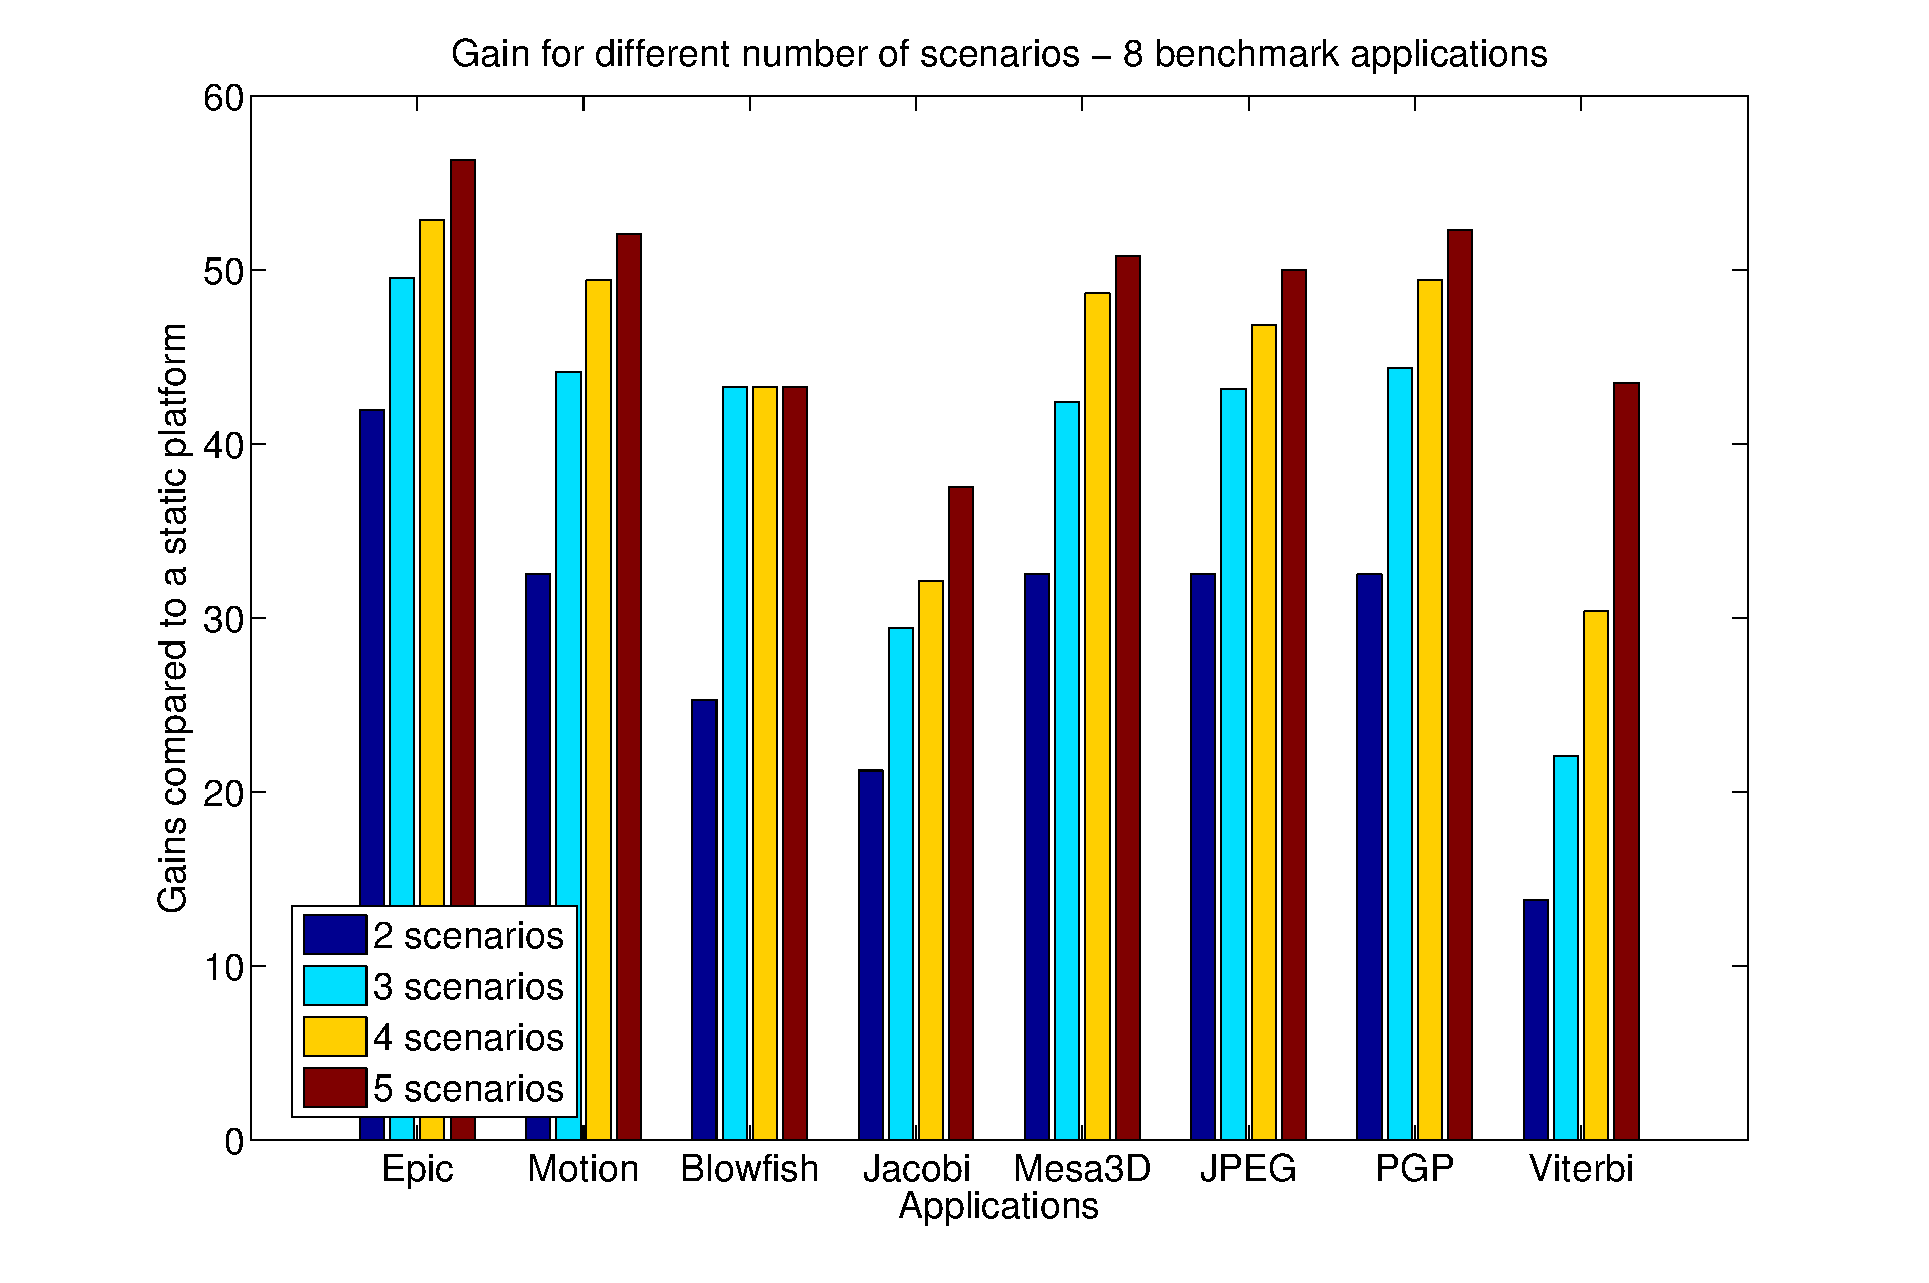
\includegraphics[width=\textwidth]{B/Images/6appsGains.pdf}
\caption{Energy gain for increasing number of system scenarios - Static platform corresponds to 0\%}
\label{fig:gains}
\end{figure}

The introduction of a second system scenario results in energy gains between 15\% and  40\%  for the tested applications. Depending on the application's dynamism the maximum reported energy gains range from around 35\% to 55\%. As expected according to the categorisation presented in subsection~\ref{sec:applicationsB}, higher energy gains are achieved for applications with more dynamic memory requirements, i.e., bigger difference between the minimum and maximum allocated size. The maximum gains for JPEG, motion estimator, mesa 3D and PGP are around 50\% while blowfish, jacobi, and Viterbi decoders are around 40\%. 

As the number of system scenarios that are implemented on the memory subsystem increases, the energy gains improve since variations in memory requirements can be better exploited with more configurations. The switching cost also increases for an increasing number of system scenarios due to the increasing frequency of platform reconfiguration. This overhead reduces the achieved gain, but for up to 5 scenarios we still see improvements for all but one of our benchmarks. The switching cost is below 2\% even for a platform with 5 memory banks in all cases. The most efficient of the tested organisations for each benchmark are presented in Fig.~\ref{fig:banks}, where each memory bank is depicted with a different colour and each length is proportional to the memory bank size. The blowfish decoder is the only benchmark that has only 3 banks in its most efficient memory organisation.

\begin{figure}[!t]
\centering
%\includegraphics[angle=270, width=0.47\textwidth]{Images/banks.ps}
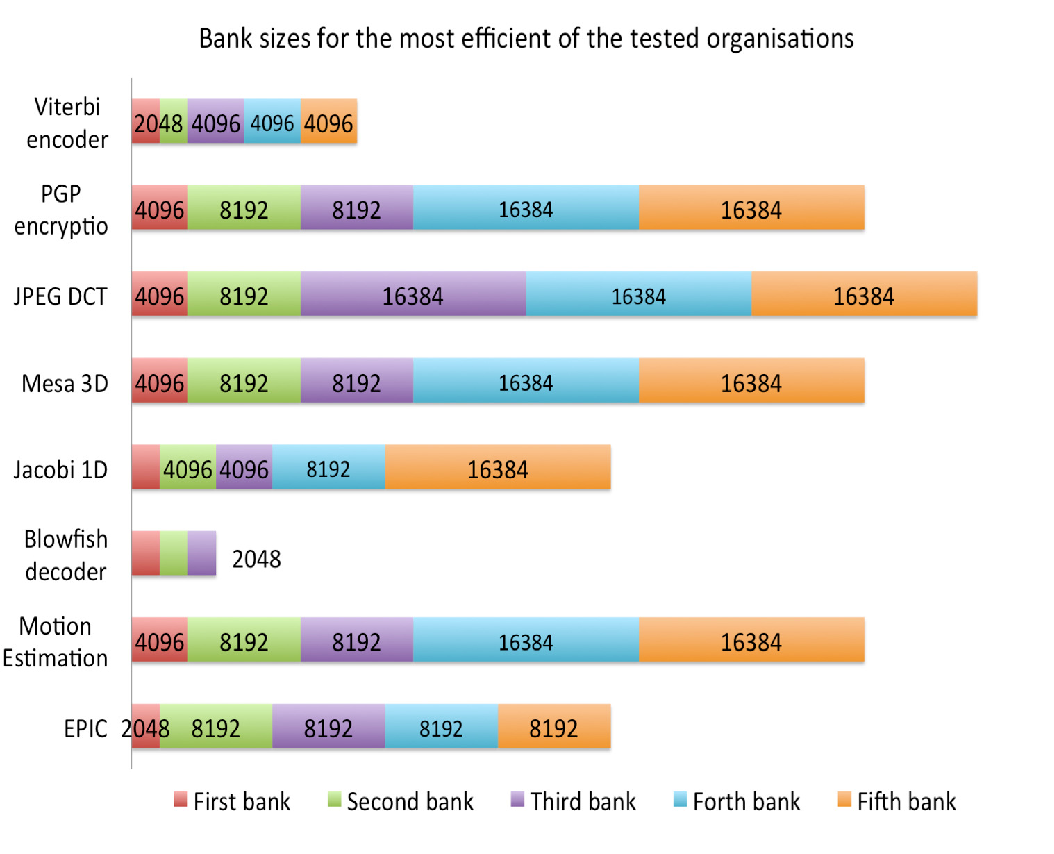
\includegraphics[width=\textwidth]{B/Images/banks2.pdf}
%\psfig{file=Images/banks.ps, angle=270, width=0.47\textwidth}
\caption{Bank sizes for the most efficient of the tested organisations for each benchmark}
\label{fig:banks}
\end{figure} 

Comparative results from applying a use case scenario approach as a reference are presented in Fig.~\ref{fig:usecase}. Reported energy gains for both use case scenarios and system scenarios are given assuming a static platform as a base (0\%). Use case scenarios are generated based on a higher abstraction level that is visible as a user's behaviour. For example, use case scenarios for image processing applications generate three scenarios, if large, medium and small are the image sizes identified by the user. In general, use case scenario identification can be seen as more coarse compared to identification on the detailed system implementation level.
 
\begin{figure}[!t]
\centering
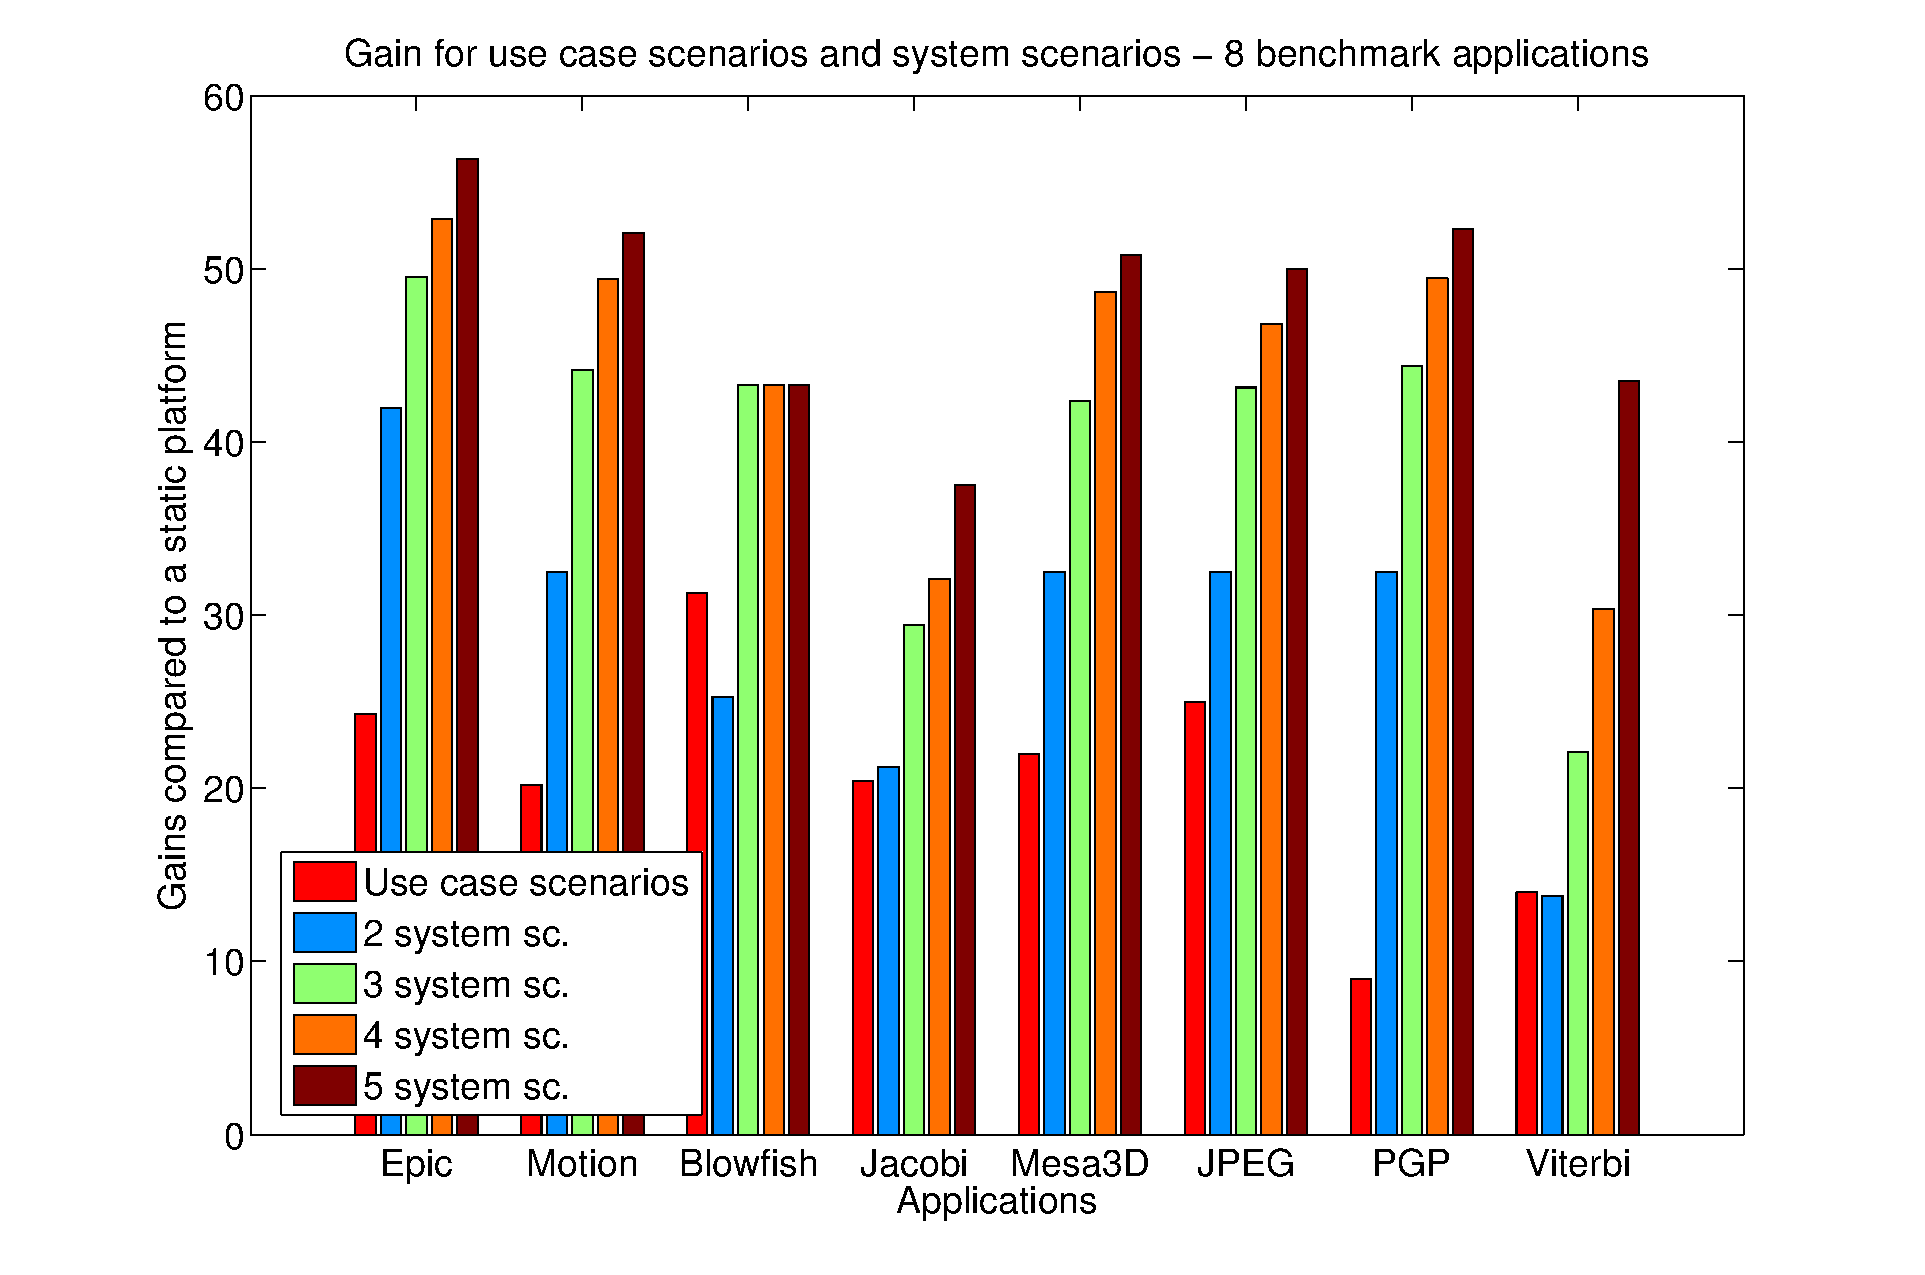
\includegraphics[width=\textwidth]{B/Images/usecase.pdf}
%\includegraphics{file=Images/usecase.eps, width=0.47\textwidth}
\caption{Energy gain for use case scenarios and system scenarios}
\label{fig:usecase}
\end{figure}

\section{Conclusion}
%\label{sec:conclusion}

The scope of this work is to apply the memory-aware system scenario methodology to a wide range of multimedia application and test its effectiveness based on an extensive memory energy model. The results demonstrate the effectiveness of the methodology reducing the memory energy consumption between 35\% and 55\%. 

\bibliographystyle{plain}
\bibliography{reference}